\section{Durchführung}
\label{sec:Durchführung}

% Was wurde gemessen bzw. welche Größen wurden variiert?

Das Experiment wird nach \autoref{fig:messung} aufgebaut.

\begin{figure}
    \centering
    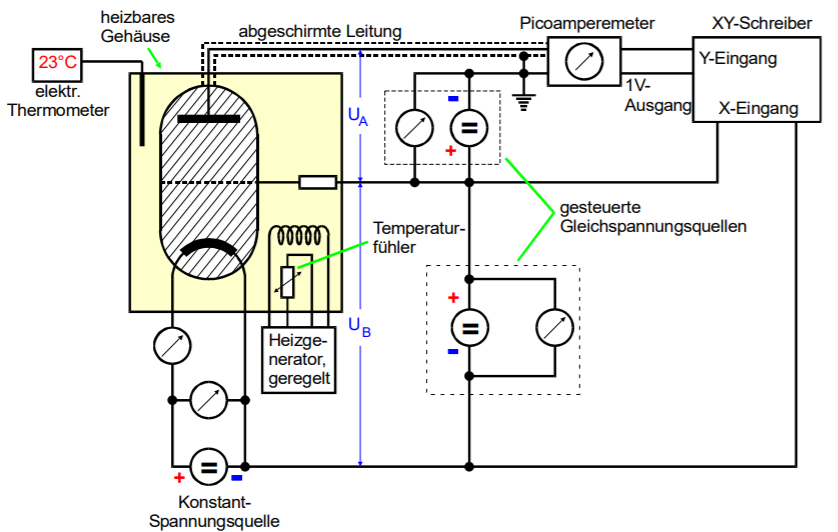
\includegraphics[width=0.6\textwidth]{images/bild5.png}
    \caption{Schaltungsbild des Franck-Hertz-Versuchs.\cite{V601}}
    \label{fig:messung}
\end{figure}

In der ersten Messreihe wird die Energieverteilung der Elektronen bestimmt.
Dafür wird $U_\text{B}$ konstant auf $\SI{11}{\volt}$ eingestellt und $U_\text{A}$ von null aus zu einem Maximalwert erhöht.
Die detektierte Spannung an der Auffängerelektrode wird mit einem Picoamperemeter angezeigt.
Für die Darstellung wird ein XY-Schreiber verwendet, wobei $U_\text{A}$ an den X-Eingang angeschlossen wird, und $I_\text{A}$ an den Y-Eingang.
Die Messung wird bei Raumtemperatur durchgeführt.
Es ist darauf zu achten, dass bei $U_\text{A} = 0$ ein maximaler Strom von $\SI{50}{\nano\ampere}$ bis $\SI{500}{\nano\ampere}$ fließen soll. 
Falls das nicht der Fall ist, wird die Spannung der Glühkathode dahingehend verstellt.
Während oder nach dem erstellen des XY-Schreiber-Bilds werden einige Messpunkte als Referenzwerte eingetragen, um die Auswertung möglich zu machen.

Die eigentliche Messung der Franck-Hertz-Kurve findet bei $T = \SI{180}{\celsius}$ statt.
$U_\text{A}$ wird auf $\SI{-1}{\volt}$ eingestellt.
Hier wird $U_\text{B}$ an den X-Eingang gelegt und von null aus zum Maximalwert geregelt.
Auch hier werden verschiedene Messpunkte beschriftet.
Eine optimale Auswertung gelingt, wenn der XY-Schreiber das Blatt möglichst effizient nutzt.
